\documentclass[11pt,twocolumn]{article}

% Pretty much all of the ams maths packages
\usepackage{amsmath,amsthm,amssymb,amsfonts}

%page layout
\usepackage[margin=1in]{geometry}

% Removes paragraph indentation (not needed most of the time now)
\usepackage{parskip}

% Allows inclusion of graphics easily and configurably
\usepackage{graphicx}

% Provides ways to make nice looking tables
\usepackage{booktabs}

% Allows you to rotate tables and figures
\usepackage{rotating}

\usepackage{titlesec}

\usepackage{mathptmx}
\usepackage{chemfig}
\usepackage{tikz}
\usetikzlibrary{arrows,positioning,shapes.geometric,shapes.misc}

% Allows shading of table cells
\usepackage{colortbl}
% Define a simple command to use at the start of a table row to make it have a shaded background
\newcommand{\gray}{\rowcolor[gray]{.9}}

\usepackage{textcomp}

% Provides commands to make subfigures (figures with (a), (b) and (c))
\usepackage{subfigure}

% Typesets URLs sensibly - with tt font, clickable in PDFs, and not breaking across lines
\usepackage{url}

% Makes references hyperlinks in PDF output
\usepackage{hyperref}


% Provides good access to colours
\usepackage{color}
\usepackage{xcolor}

% Vastly improves the standard formatting of captions
\usepackage[margin=10pt,font=small,labelfont=bf, labelsep=endash]{caption}

\titleformat{\subsection}
{\normalfont\itshape}{\thesubsection}{1em}{}

%opening
\title{A Novel Orientation-Dependent Potential for \\Protein Structure Prediction}
\author{Venkatesh Sivaraman, Bexley High School}

\begin{document}

\maketitle

\raggedbottom

\begin{abstract}
\end{abstract}

\section{Introduction}
Predicting the 3-dimensional structure of proteins remains a challenge despite advances in theory and computational power over the past three decades.
Modeling protein folding has numerous biological applications, including active site detection, protein design, and visualizing the formation of complexes, ligand binding, and protein-membrane interactions \cite{baker2,kouza,monticelli}.
However, the most detailed simulations must incorporate hundreds of atoms at picosecond time intervals, which currently prohibits the timescale on which these simulations can be computed.
Therefore, many biological applications would benefit from a coarse-grained approach that preserves as much detail as possible from atomistic methods.

The thermodynamic hypothesis, proposed by Anfinsen, stipulates that the native structure corresponds to the free energy minimum of all possible conformational states of the protein \cite{anfinsen}.
Therefore, the crux of structure prediction methods is to accurately express the energy of a protein in a given state. 
Energy functions generally fall under two categories: ``physics-based'' and ``knowledge-based potentials'' \cite{lu}.
Physics-based potentials and force fields, such as CHARMM \cite{brooks}, AMBER \cite{amber}, and GROMOS \cite{gromos}, evaluate conventional bonded and nonbonded energy terms (e.g. bond stretch, dihedral angle, and Coulombic potentials) for all atoms in a structure \cite{brooks2}.
These atomistic potentials can be made coarse-grained by modeling residues as one or a few particles, or by considering groups of residues as rigid subparts \cite{basdevant,potestio,enciso,monticelli}.
However, physics-based potentials necessitate either the inclusion of explicit solvent molecules in the simulation \cite{onufriev} or the use of implicit solvent techniques such as the generalized Born/solvent-accessible surface area (GBSA) model \cite{feig,roux}.
This tends to render all-atom force fields computationally inefficient if not intractable in large-scale molecular dynamics (MD) applications.

The second type of energy function, knowledge-based potentials (KBPs), have developed as an approximative substitute for physics-based potentials and are more efficient at comparative tasks such as the gapless threading problem, which involves choosing the most likely native structure out of a series of candidates \cite{thomas2}.
KBPs, also known as ``statistical potentials,'' are based on statistical analysis of known protein structures rather than distinct physical or chemical interactions. 
The use of KBPs was pioneered by Tanaka and Scheraga \cite{tanaka}, then Miyazawa and Jernigan \cite{miyazawa}, who estimated inter-residue interaction energies by counting contacts (pairs of residues located within a certain cut-off distance of each other) between types of amino acids in known protein structures.

The underlying assumption in assembling these statistical energy functions is that the known structures, usually obtained by X-ray crystallography or NMR, correspond to equilibrium states \cite{buchete2003}. 
As a consequence, the frequency of a local structure (e.g. a contact, distance, or relative orientation) can be related to its conformational energy according to the Boltzmann distribution.
This yields the following commonly-used expression for calculating energies by statistical analysis:

\begin{equation}
E(s) = -kT\ln{P(s)}
\label{boltzmann_device}
\end{equation}

where $s$ represents a local conformation, $k$ is Boltzmann's constant, $T$ is the temperature, and $P(s)$ is the probability of the state occurring in equilibrium \cite{sippl}.

Beyond contact potentials, various methods have also been developed based on the distribution of Euclidean distances between residues, such as DOPE \cite{shen}, DFIRE \cite{zhou}, GOAP \cite{zhou2}, and others \cite{lu,zhang}.
A few studies have incorporated anisotropic factors by comparing the orientations of the sidechains \cite{zhang3,mukherjee} or by measuring polar, spherical and/or Euler angles between two contacting residues \cite{miyazawa2,buchete2003}. 
In general orientation-dependent energy terms based on bond angles are also combined with dedicated distance-dependent components, though the additivity of statistical energy terms concerning orientation and distance has been questioned \cite{shen}.
Moreover, these statistical potentials may be limited by their concern with only the backbone or the sidechains, as well as failure to consider the tendency of hydrophobic residues to move toward solvent-inaccessible regions \cite{mullinax}.

This paper presents a new anisotropic statistical potential, called Segmented Positional Analysis of Residue Contacts (SPARC), that addresses concerns with other statistical methods by generalizing the expression of amino acid orientations through local coordinate system transformations.
We describe the methods used to derive SPARC from the database of known protein structures, as well as a ``coordination number''-based implicit solvent interaction model extended from Miyazawa and Jernigan \cite{miyazawa}.
SPARC is then evaluated based on its performance on the gapless threading problem in comparison to other statistical potentials, and tested in a new segmented dynamic Monte Carlo simulation of protein folding.

\section{Methods}

\begin{figure}
	\begin{center}
		\begin{tikzpicture}
		\setbondoffset{3pt}
		\draw[->,>=stealth] (0.2,0) -- (2.5,0) node [right,black] {\textbf{j}};
		\draw (-0.5,0) -- (-2.5,0);
		\draw[->,>=stealth] (0,2.1) -- (0,2.5) node [above,black] {\textbf{k}};
		\draw (0,-0.4) -- (0,-2.3);
		\draw[->,>=stealth] (-0.3,-0.3) -- (-1.8,-1.8);
		\node at (-2, -2) {\textbf{i}};
		\draw (0.2,0.2) -- (1.7,1.7);
		\node at (0,0) {\chemfig[][scale=1.6]{C_\alpha(-[2]R)(<[:240]H)(>:[:340]C)(>:[:200]N)}};
		\end{tikzpicture}
	\end{center}
	\caption{The core structure of an amino acid around the $\alpha$-carbon. We utilize the bond angles predicted by VSEPR theory to assign each amino acid a local coordinate system.}
	\label{aminoacid_axes}
\end{figure}

\subsection{Construction of local coordinate system}
Given a protein of $n$ amino acids, we can assign a Cartesian local coordinate system (LCS) to each residue to quantify its orientation with respect to an arbitrary global coordinate system (GCS).
To determine a set of basis vectors that is consistent across all 20 sidechain types, we turn to the ideal bond angles predicted by valence-shell electron-pair repulsion (VSEPR) theory \cite{gillespie}.
As shown in Fig. \ref{aminoacid_axes}, the bond geometry around the C$_\alpha$ atom is approximately tetrahedral, with bond angles of $\cos^{-1}{1/3}\approx 109.5^\circ$.

Defining $\textbf{n}$ and $\textbf{c}$ as the normalized vectors in the GCS pointing from C$_\alpha$ to the amine nitrogen and carbonyl carbon, respectively, we define $\textbf{j} \equiv \pm(\textbf{n} - \textbf{c})$, with the sign that minimizes the angle between \textbf{j} and \textbf{c}.
We proceed with the \textbf{k} vector, which should lie along the bond leading to the sidechain (or a hydrogen atom in the case of glycine).
Solving for \textbf{k} from the bond angles between \textbf{c} and \textbf{n} yields two solutions, each of which has an associated vector $\textbf{i}=\textbf{j}\times\textbf{k}$.
We choose the pair that maximizes the angle between \textbf{i} and \textbf{c}, which produces an LCS consistent with Fig. \ref{aminoacid_axes}.

\subsection{From orientational frequencies to energies}
The Cartesian LCS for each amino acid enables us to describe the relative orientation between any two amino acids $\textbf{p}$ and $\textbf{q}$ as simply the coordinates of $\textbf{p}$ in the LCS of $\textbf{q}$, denoted $\textbf{p}_q$, and vice versa.
To obtain a distribution of relative orientations for each sidechain type, we consider only those amino acids within a contact sphere of radius 10 \AA\, of each residue.
The orientation space is coarse-grained into intervals of 1 \AA\, for a total of 8,000 possible ``bins'' into which each relative location might fall.

As in all statistical potentials, SPARC assumes that these pairwise orientations follow the Boltzmann distribution in an ensemble of native protein structures \cite{sippl}, motivated by the fact that even at a free energy minimum, unstable \textit{local} structures can still be found.
This permits us to adapt Eq. (\ref{boltzmann_device}) to calculate a dimensionless energylike quantity from the orientational frequencies:
\begin{equation}
\displaystyle
S(\textbf{p}, \textbf{q}) \equiv -\left(\ln{\frac{f(\textbf{p}_q)f_{pq,\text{tot}}}{\bar{f}_{pq}\bar{f}_\text{tot}}} + \ln{\frac{f(\textbf{q}_p)f_{pq,\text{tot}}}{\bar{f}_{pq}\bar{f}_\text{tot}}}\right)
\label{sparc_equation}
\end{equation}
In this equation, which defines the inter-residue component of SPARC, $f(\textbf{p}_q)$ refers to the frequency of an interaction between amino acids of type $p$ and $q$ with that particular relative location. 
$\bar{f}_{pq}$ represents the mean frequency over all bins, and $f_{pq,\text{tot}}$ the total number of contacts for these amino acid types (e.g. alanine and tyrosine, glycine and glutamine, etc.).
$\bar{f}_\text{tot}$ is the mean number of contacts over all combinations of amino acid types.
The result of this formulation is that contacts whose relative orientations are above average receive a more negative (stable) score.
Furthermore, for a perfectly ``average'' orientation, a more negative score will result if contacts between amino acid types $p$ and $q$ are more frequent in the native ensemble.

Another important consideration when constructing SPARC was chain connectivity, since it is presumed that amino acids adjacent to each other along the peptide backbone interact differently (due to the presence of connecting covalent bonds) than non-consecutive residues.
Therefore, the consecutive and non-consecutive amino acids found within the 10-\AA\, shell were separated and analyzed separately, producing two distinct score functions $S_c$ and $S_{nc}$.

\subsection{Solvent interaction model}
In a simplified sense, the intermolecular interactions that determine the stability of a protein structure can be decomposed into those between residues and those between residues and the solvent.
The latter interactions cannot be modeled by orientation in an implicit solvent, so they are collectively modeled by SPARC in terms of the ``coordination number'' or packing density of the residues.
This approximation is similar to the coordination numbers used by Miyazawa and Jernigan \cite{miyazawa}; however, instead of calculating the values indirectly from the volume of each residue type, we are able to count the number of amino acids within the contact sphere because of the large sample size and variety in our structures (see section \ref{materials}).
The analog for eq. (\ref{sparc_equation}) for the solvent interactions then becomes

\begin{equation}
S_{\text{solv}}(\textbf{p})\equiv -\ln{\frac{f(|A_p^*|)}{\bar{f}_p}},
\label{solvent_equation}
\end{equation}

where $A_p^*$ represents the set of amino acids within the cutoff distance and $\bar{f}_p$ the mean frequency over the possible coordination numbers for amino acid type $p$.
The energylike quantities represented by $S_c$, $S_{nc}$, and $S_\text{solv}$ are finally added together to produce an overall SPARC score value.

\subsection{Dynamic Monte Carlo simulation}
The statistical nature of SPARC makes it especially conducive to a Markov chain Monte Carlo (MCMC) simulation because it provides direct local stability comparisons which can be used to sample the conformational space.
Monte Carlo simulations have been used with some frequency to predict protein structure \cite{kolinski,enciso}, though not as often or as successfully as deterministic molecular dynamics (MD).
The most widely-used MCMC technique is the Metropolis-Hastings algorithm, which uses a weighted form of rejection sampling to approximate a distribution over a large number of iterations \cite{metropolis}.
We utilize a modified version of the Metropolis-Hastings algorithm based on the distribution of relative orientations in SPARC.

An overview of the simulation algorithm is presented in Fig. \ref{flowchart}.

\begin{figure}
\begin{center}
	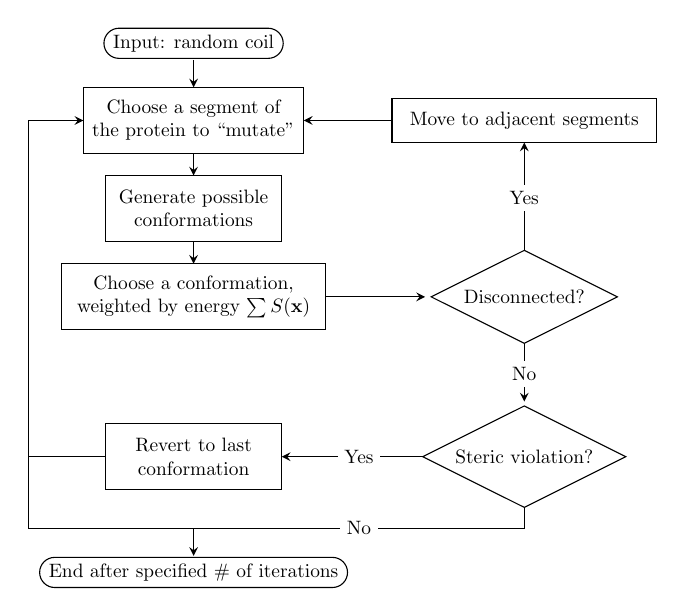
\begin{tikzpicture}[scale=0.7, every node/.style={scale=0.7}]
	\draw [->, >=stealth] (0,-1.5) -- (0, -2);
	\draw [->, >=stealth] (0,-2.5) -- (0, -3.6);
	\draw [->, >=stealth] (0,-4.5) -- (0, -5.2);
	\draw [->, >=stealth] (0,-5.8) -- (4.2, -5.8);
	\draw [->, >=stealth] (6, -5.8) -- (6, -3);
	\draw [->, >=stealth] (3.6, -2.6) -- (2, -2.6);
	\draw [->, >=stealth] (6, -6.6) -- (6, -7.7);
	\draw [->, >=stealth] (6, -8.7) -- (1.6, -8.7);
	\draw (6, -8.7) -- (6, -10) --(-3, -10)  -- (-3, -8.7);
	\draw [->, >=stealth] (0, -8.7) -- (-3, -8.7) -- (-3, -2.6) -- (-2, -2.6);
	\draw [->, >=stealth] (0, -10) -- (0, -10.5);
	
	\node [draw, rounded rectangle, fill=white] at (0, -1.2) {Input: random coil};
	\draw [fill=white,text width=3.8cm,align=center] (-2,-2) rectangle (2,-3.2) node[pos=.5] {Choose a segment of the protein to ``mutate''};
	\draw [fill=white,text width=3cm,align=center] (-1.6,-3.6) rectangle (1.6,-4.8) node[pos=.5] {Generate possible conformations};
	\draw [fill=white,text width=4.5cm,align=center] (-2.4,-5.2) rectangle (2.4,-6.4) node[pos=.5] {Choose a conformation, weighted by energy $\sum S(\textbf{x})$};
	\node [draw, diamond, fill=white, aspect=2] at (6, -5.8) {Disconnected?};
	\node [fill, white, rectangle, text=black] at (6, -4) {Yes};
	\node [fill, white, rectangle, text=black] at (6, -7.2) {No};
	\node [draw, diamond, fill=white, aspect=2] at (6, -8.7) {Steric violation?};
	\draw [fill=white,text width=4.4cm,align=center] (3.6,-2.2) rectangle (8.4,-3) node[pos=.5] {Move to adjacent segments};
	\node [fill, white, rectangle, text=black] at (3, -8.7) {Yes};
	\node [fill, white, rectangle, text=black] at (3, -10) {No};
	\draw [fill=white,text width=3cm,align=center] (-1.6,-8.1) rectangle (1.6,-9.3) node[pos=.5] {Revert to last conformation};
	\node [draw, rounded rectangle, fill=white] at (0, -10.8) {End after specified \# of iterations};
	\end{tikzpicture}
\end{center}
	\label{flowchart}
	\caption{An overview of a Markov chain Monte Carlo (MCMC) simulation algorithm developed using SPARC. The procedure is similar to that of the Metropolis-Hastings algorithm in that new structures are sampled so that better-scoring conformations are chosen more often.}
\end{figure}

\subsection{Materials and software}
\label{materials}
All calculations and programs were run on an off-the-shelf laptop computer and a desktop.
Written in Python 2.7 and comprising about 6,000 lines of code, this first version of the SPARC software contains tools for reading and writing PDB files, analyzing structures for orientation data directly from the Protein Data Bank, and running the dynamic Monte Carlo simulations as well as other utilities, with all modules designed to be subclassable and extendible for future modifications.

To calculate the orientational frequencies, a large dataset of native protein structures determined using X-ray crystallography (91,995 total structures) was obtained from the Protein Data Bank.

\section{Results}

\section{Discussion}

\section{Conclusion}

\bibliographystyle{abbrv}
%\nocite{*}
{\footnotesize \bibliography{biblio.bib}}
\end{document}
